\documentclass{jsarticle}
\usepackage[dvipdfmx,hiresbb]{graphicx}

\begin{document}

\title{音楽再生と時間の関係}
\author{藤賀雄太}
\date{2012年12月1日}
\maketitle

\section{イントロダクション}
\subsection{世の中の現状分析}
音楽記録メディアはデジタル化によって小型化が進み、携帯可能な小さな機器(以後、モバイルプレイヤーと呼ぶ)になった。
ウォークマンやiPodを代表とする再生専用機器は広く普及したが、最近では、携帯電話と一体型になっているものも広く普及しており、音楽再生機器をどこでも持ち歩けるようになった。
また、スピーカーではなく、ヘッドホンで聴く場合、自分だけ聴くことができるため、例えば電車の中などの公共空間で聴くことや、学校の授業の合間の時間にすぐに取り出して聴けるようになった。そのため、音楽を聴く場所と時間に制約がなくなり、どんな時刻でも、どこにいても、好きな楽曲を聴くことができるようになった。

\subsection{現状分析から見えてくる問題点}
時間によって違うから、もっと動的なシーンに動的に対応しないとついて行ってない感じよね。これじゃないっていうか、そういうかんじよ。

\subsection{現状分析から見えてくるチャンス}
一方、生活のコンテキスト(時間や場所の情報)から音楽をリコメンドするものはあまりみつけられなかったが、楽曲の音楽の情報自体にアクセスするのではなく、楽曲が再生される状況の関係性から楽曲を分析することができるのではないかと考えた。リコメンドサービスにおいてはジャンルによって推薦するものが多いが、ユーザーが考える音楽ジャンルと必ずしも一致しているとは限らない。そこで、時間という属性で音楽をマクロに分けて、ユーザーが音楽を再生するときの、その時刻の情報によって、音楽を推薦できないかと考えた。

\subsection{特に注目する問題ひとつ(研究課題)}
音楽再生時のユーザー自身の状況から、音楽を推薦するために、いくつかの要素を抽出して、予備的な音楽再生ソフトを自作して、自身で使ってみたり、プレゼンやデモを通して第三者からもフィードバックをもらった。
\begin{enumerate}
\item
場所

GPSを利用して音楽の履歴情報を地図にプロットしていき、再生時の位置情報により、音楽を推薦する方式。
\item
時刻

音楽の再生時刻をから推薦する方式。
\item
シーン

音楽を再生する際にシーンを選択してもらうことによりシーンにあった音楽を推薦する方式。
\end{enumerate}

正式ではないものの、以上の予備的なソフトを体験してみて、場所については、場所によって異なる音楽を聴いていることもあったが、それは、場所自体に直接的な意味合いがあるというよりも、その時刻にその場所にいることが多いという、間接的な関係であった。時刻に比べて相関が薄かった。例えば、移動中であったときは、状況は移動中であるだけなのにもかかわらず、移動している場所にちりばめられるといったことが起こった。また、同じ場所であっても、休憩中や、作業中などの様々なシーンに応じて音楽を選んでいる場合でも、一元化されてしまうといった問題点もあった。
シーンを選ぶものは、ユーザー自身で音楽のモードを選んで、選択してもらうことから、実際にはプレイリストを自作する行為に似ており、リコメンドサービスとしてのメリットが小さくなってしまった。また、なぜ、そのシーンを選んだのかといった属性が不明瞭なため、膨大な学習期間を要することも問題だった。
時刻に関しては、すでに述べた、場所、シーンの両方ともに関係しており、音楽をかける際に、ユーザーの状況を説明するのに、最も基本的な要素であり、直接的だったため、本研究では時間について特に注目して調べることにした。このことにより、この研究成果が、場所情報と組み合わせることで状況をより正確に推測したり、シーンを時間から推測したりといった拡張性に期待したいと考えた。


\subsection{既知の壁}
人によって、生活が不規則な人もいると容易に推測できるために、時間によって、傾向が出ないことも考えられる。必ずしも。時間と音楽の再生に相関がある人ばかりではないことも留意しつつ、調べる必要がある。そのため、音楽の再生時刻だけでなく、普段の生活がどのようになっているのかを直接知る必要がある。また、ランダム再生(=シャッフル再生)機能が広く普及しており、再生履歴も一元的にユーザーによる積極的な選択としてみなすことが出来ない場合も注意する必要がある。また、ソフトの仕様により、履歴情報が全て記録されていない場合があり、今回使用したAppleによるiTunesという音楽再生プレイヤーは、ひとつの楽曲に対して、最後に再生した時刻だけしか記録されていない。全てを保存するアプリケーションを自作することも可能だったが、その場合、従来の音楽再生の体験自体を大きく変化させてしまうことによって、従来の履歴情報を取得することが困難になると考えたため、この点においては妥協してiTuensを使用することにした。
また、今回はAppleのiTuensという音楽再生プレイヤーに限定して分析した。そのため、実際に音楽を再生するまでにかかる工程が、iTuensのユーザーインターフェースに依存してしまうため、他の音楽再生プレイヤーで得られた履歴情報とは偏りが出来る可能性がある。ジャンル名を取得できていない楽曲もあり、またユーザーが手動で設定しなくても、iTunesが自動的につけるために、ユーザーが考える音楽ジャンルとくくりと、必ずしも合致するとも限らない。
\subsection{先行研究}
産総研の後藤真孝さんのMusicreamのように、インターフェースによって音楽を選択する支援をするものや、楽曲のジャンルの関連性を取得するgeniusなどのサービス、また、ユーザーが楽曲から受ける印象を集めることで、音楽の印象から、気分にあった音楽を選ぶことのできるmusicoveryなどのサービスがある。

\subsection{研究動機}

以前は例えば自宅で夜、音楽鑑賞するといった決まった状況で聴いていたため、音楽を再生する状況に外的な別段の変化はなかった。
しかし、モバイルプレイヤーにおける音楽の再生は、場所や時間を選ばない。そのため、モバイルプレイヤーの使用者は様々な場所や時間において、自分で音楽を再生する音楽を選択する必要がでてきた。
ユーザーは、状況が変化すると、音楽を再生する同期や気分などに差が大きく出ると思われる。
そこで、私は、外的な状況の変化に対して、音楽の再生がどのように変化しているのかを調べることにした。
\subsection{方針}
本研究では特に時刻に注目して、時刻によって音楽の聴き方がどのように変化するのかを調べた。
時刻に注目した理由は以下の通りである。
\begin{itemize}
\item
規則的、周期的である。ほとんどの場合、朝は自宅から始まり、夜は再び、自宅にもどる。その時間も人によってではあるが、パターン化されていると考えられる。そのため、時刻だけからもある程度、人の営みを推測することができそうだと推測できた。
\item
音楽と相関がありそうである。現状で、朝の音楽や、オールナイトコンサート、夜のジャズクラブなど、時間を冠した音楽のシーンは見慣れている。そのため音楽には時間的な要素が存在していると予測できた。
\end{itemize}

\subsection{期待される成果}
この研究が音楽の自動選曲システムの向上に貢献できればと考える。研究の結果、時間情報はfoobarでした。
\subsection{キーワード}
iTunes, iPod, 時間情報, レコメンドサービス, ライフログ

\section{分析手順}
\begin{enumerate}
\item
被験者10名(iTunesをいつも利用して音楽を聴いている大学生)から履歴ファイル(xmlファイル)をメール添付でもらう。

\item
被験者に自分の生活を曜日毎にアンケートシートに書いてもらう。
\begin{figure}[htbp]
\begin{center}
\fbox{
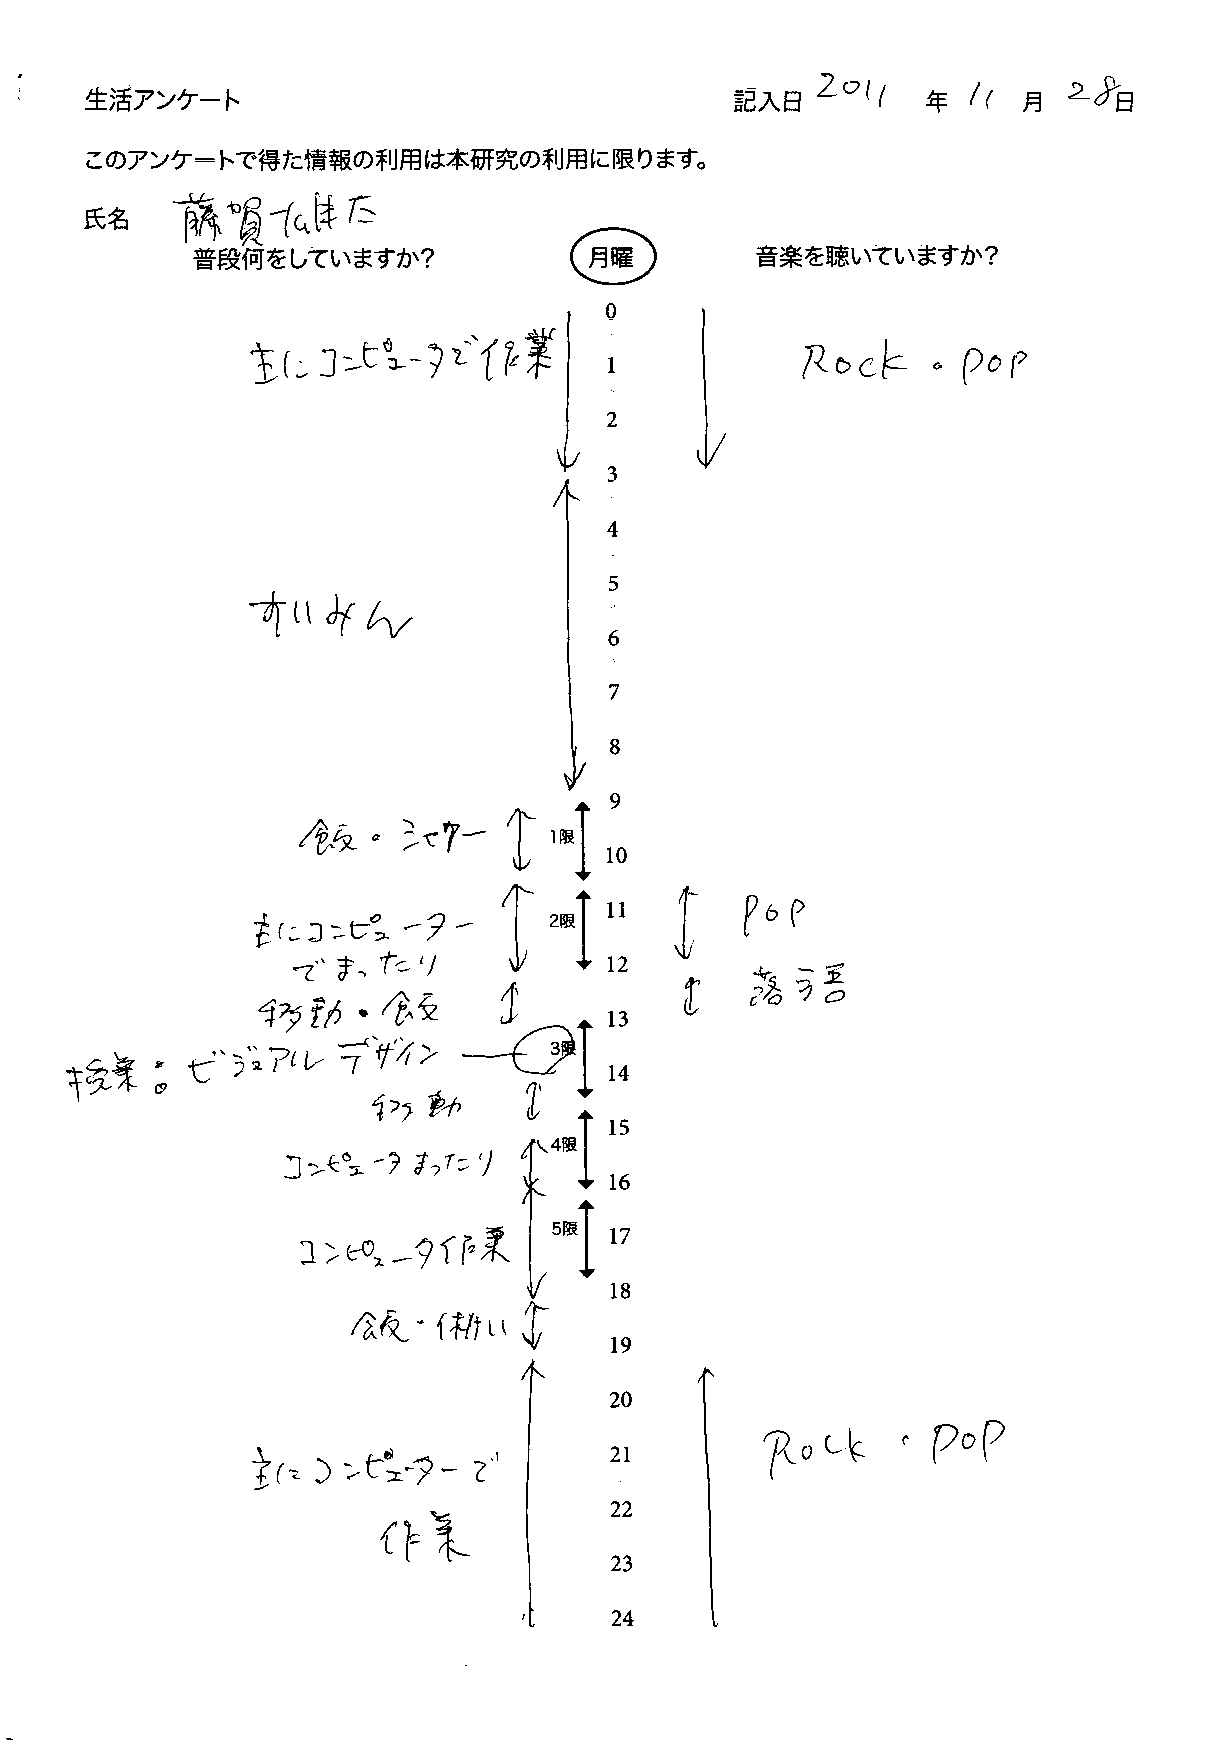
\includegraphics[width=7cm]{musicLifeSheet_sample.pdf}
}
\caption{アンケートシートのサンプル}
\end{center}
\end{figure}

被験者に渡したのは、0時から24時までを30分刻みで目盛りを付けたもので、普段の生活と、普段の音楽聴取を記入してもらうもので、月曜日から日曜日までの合計7枚のものである。
不規則な生活、気まぐれな音楽再生など、毎週規則正しく定期的に書けない部分も備考として記入してもらう。
なお、iTunesをシャッフルで聴いたかどうかは、iTunesに記録されていないため、備考に書いてもらう。
\item
pythonを用いて、履歴ファイルから、以下の情報だけを読み取って、テキストファイルに書き出す。
\begin{itemize}
\item
楽曲のジャンル
\item
最後に聴いた日付・時間
\item
再生回数
\end{itemize}

\item
Rを用いて、2でつくったテキストファイルを読み込んで、一度以上再生された楽曲について、曜日毎に分類し、さらに、0時から24時まで1時間刻みのヒストグラムをつくる。そして、ヒストグラムのデータをcsvファイルとして保存する。なお、ヒストグラムを画像ファイル(pngデータ)として書き出す。

\item
openFrameworksを用いて、csvファイルから、0時から24時まで30分刻みのヒストグラムを月曜から日曜までの累積棒グラフの形式でつくる。棒グラフの棒の数は、24(1時間刻み)*7(月曜から日曜)=168本になる。総合再生回数がベスト5のものだけをカラーにして、それ以外をその他としてグレーで描画した。

\begin{figure}
\begin{center}
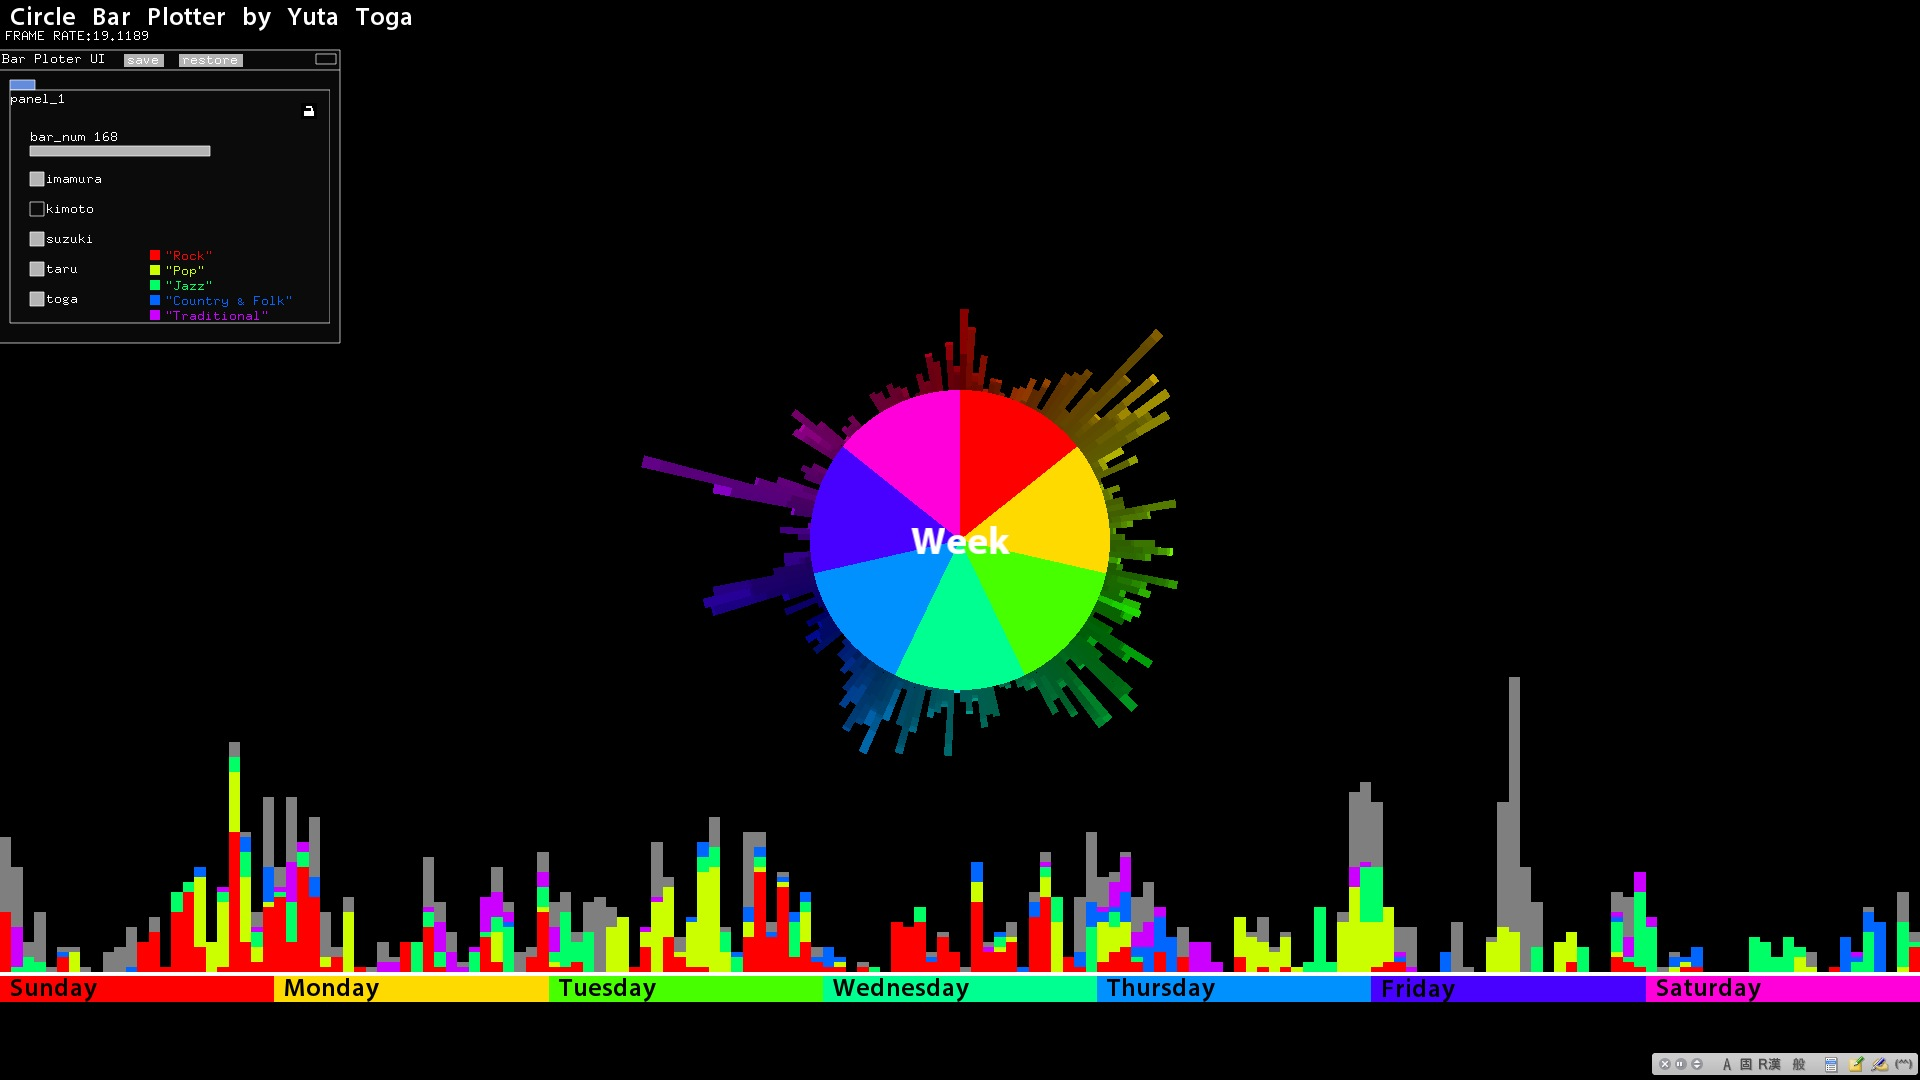
\includegraphics[width=14cm]{graph_sample.jpg}
\caption{分析結果のグラフ}
\end{center}
\end{figure}

\item
ヒストグラムの見た目から、聴いている音楽と、時間に相関があるかを調べる。
\item
被験者のアンケートシートで得た情報と、xmlファイルから読み取ったものとの比較を行う。
\item
質問があったらインタビューを行う。

\end{enumerate}
\subsection{グラフについて}
グラフは自作したプログラムによって表示している。
表示するグラフは主に3通りである。

\paragraph{ほげほげほげ} ほげの用途について解説すると、・・・ほげの用途について解説すると、・・・ほげの用途について解説すると、・・・ほげの用途について解説すると、・・・ほげの用途について解説すると、・・・ほげの用途について解説すると、・・・ほげの用途について解説すると、・・・ほげの用途について解説すると、・・・ほげの用途について解説すると、・・・ほげの用途について解説すると、・・・ほげの用途について解説すると、・・・


\begin{description}
\item[ほげ] ほげの用途について解説すると、・・・ほげの用途について解説すると、・・・ほげの用途について解説すると、・・・ほげの用途について解説すると、・・・ほげの用途について解説すると、・・・ほげの用途について解説すると、・・・ほげの用途について解説すると、・・・ほげの用途について解説すると、・・・
\paragraph{ほげ} ほげの用途について解説すると、・・・ほげの用途について解説すると、・・・ほげの用途について解説すると、・・・ほげの用途について解説すると、・・・ほげの用途について解説すると、・・・ほげの用途について解説すると、・・・ほげの用途について解説すると、・・・ほげの用途について解説すると、・・・ほげの用途について解説すると、・・・ほげの用途について解説すると、・・・ほげの用途について解説すると、・・・

\item[ほげほげほげ] ほげの用途について解説すると、・・・ほげの用途について解説すると、・・・ほげの用途について解説すると、・・・ほげの用途について解説すると、・・・ほげの用途について解説すると、・・・ほげの用途について解説すると、・・・ほげの用途について解説すると、・・・ほげの用途について解説すると、・・・
\end{description}


\begin{itemize}


\item
円形の累積グラフ

長所

曜日を一周期としたときの全体の流れがわかりやすい。

短所

同じ値でも面積が中心からの距離によって異なるので、比較しにくい。


\begin{figure}[htbp]
\begin{center}
\fbox{
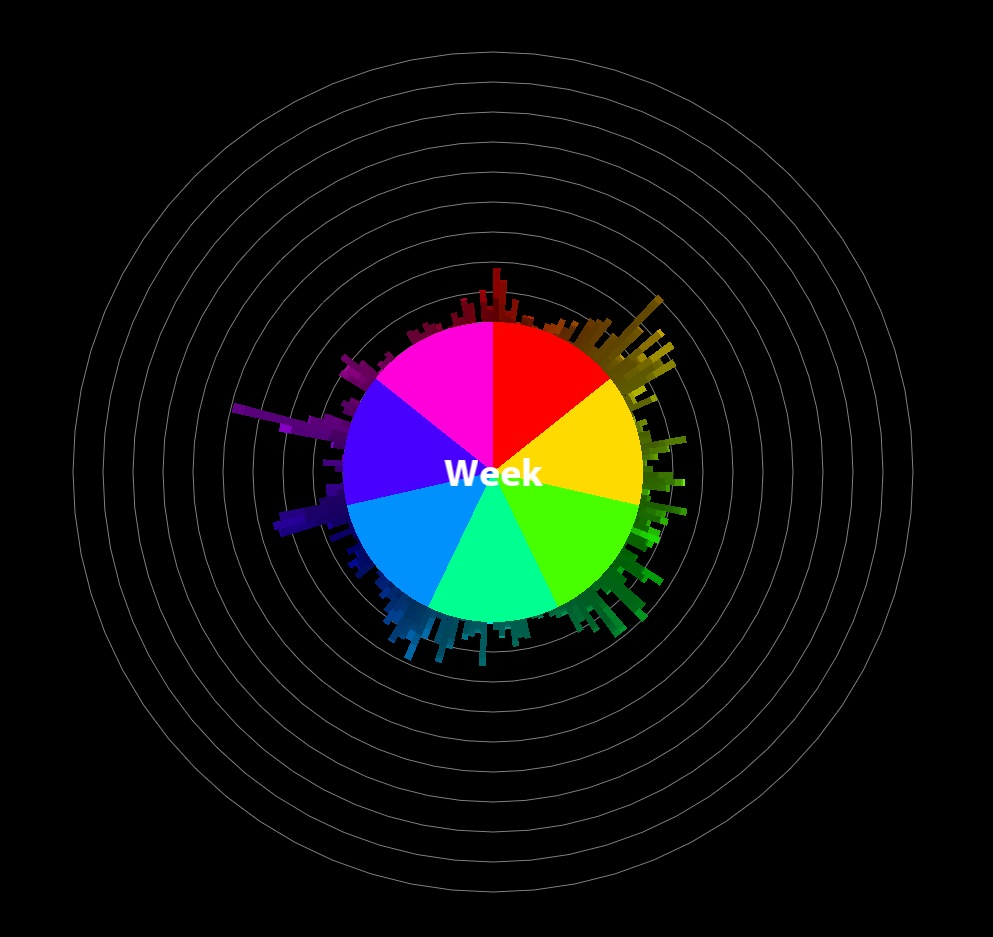
\includegraphics[width=7cm]{circleGraph.jpg}
}
\caption{累積円グラフ}
\end{center}
\end{figure}



\item
累積棒グラフ
【内容】
横軸が時間、縦軸がその時間内できかれた楽曲の回数がジャンルごとに累積表示してある。
累積する順番は、下から第一位、第二位、第三位、第四位、第五位、その他となっており、第一位から第二位に入らなかったジャンルは、その他の中に含めている。第一位から第五位はそれぞれ、5色に色分けされており、色とジャンルの対応は横に書かれている。その他は灰色にして描画されている。

長所
面積によって、比較しやすい

短所

ジャンルの比率がどのように変化しているのかは見づらい。




\begin{figure}[htbp]
\begin{center}
\fbox{
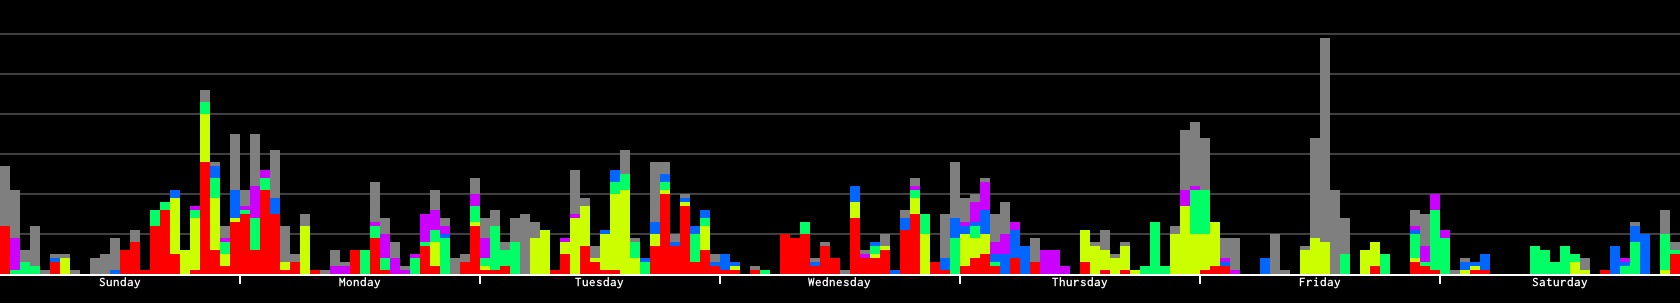
\includegraphics[width=7cm]{barGraph.jpg}
}
\caption{累積棒グラフ}
\end{center}
\end{figure}



\item
帯グラフ
【内容】
それぞれの時間に、聴いている音楽ジャンルの構成の比率を示している。横軸が時間の変化、縦軸が比率を累積表示している。
累積する順番は、上から第一位、第二位、第三位、第四位、第五位、その他となっており、第一位から第二位に入らなかったジャンルは、その他の中に含めている。第一位から第五位はそれぞれ、5色に色分けされており、色とジャンルの対応は横に書かれている。その他は灰色にして描画されている。累積棒グラフと共に表示したく無い場合は、非表示にすることもできる。

【長所】
ジャンルの構成がどのように変化しているのかを理解しやすい。


\begin{figure}[htbp]
\begin{center}
\fbox{
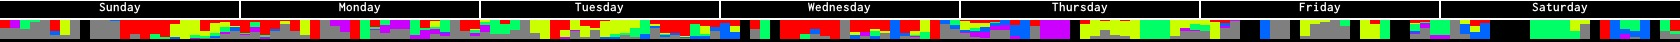
\includegraphics[width=7cm]{beltGraph.jpg}
}
\caption{帯グラフ}
\end{center}
\end{figure}

\item
iTunes上でチェックマークが入っている、すなわち、シャッフル再生で再生される可能性がある楽曲の、ジャンルのうちわけを示す円グラフ


\end{itemize}



なお、自作したグラフ表示アプリケーションは以下の機能を実装した。
\begin{itemize}
\item
フルスクリーンモードスイッチ
\item
閲覧したい人の選択スイッチ
\item
時刻によるジャンルの遷移の表示スイッチ
\item
曜日毎のジャンルトップファイブの占める割合を示す円グラフの表示スイッチ
\item
周期を合わせるために、累積棒グラフまたは、累積円グラフを回転させる機能
\item
表示するグラフのタイプ(累積円グラフまたは累積棒グラフ)を切り替えるスイッチ
\item
人毎に日曜から土曜までのそれぞれの開始時刻と終了時刻をグラフをみながら変更することのできるインターフェース。
\end{itemize}

以上により、全体の音楽の聴き方がどのように変化しているのかを累積円グラフで見た後、周期のはじまりにめぼしをつけて、累積棒グラフの始まりを左右のカーソルキーで調節して、閲覧する。ジャンルの構成の変化を調べたいときには、帯グラフを表示することにした。

\subsection{曜日について}
本研究の中での曜日は、被験者によって定義が異なる。通常であれば、1つの曜日の範囲は0時0分から24時0分であるが、本研究では、音楽を聞いて時間帯を睡眠時間と推測できるほか、アンケート用紙にて普段の睡眠時間を曜日ごとに教えてもらっているため、個人毎に起きている時間帯を曜日の範囲として定義した。そのため、曜日によっては24時間よりも長くなったり、短くなったりしている。また、0時0分からではなく、起床したと思われる時間を曜日の開始、24時0分ではなく、就寝したと思われる時間を曜日の終わりと定義した。曜日の設定は、グラフのセッティング画面より、インタラクティブに設定できるように、グラフ表示ソフトをプログラムした。その後、アンケートを見て、自己申告した情報と、音楽の履歴情報から得られた情報と異なる点、合致する点を比べた。合致すればするほど、音楽の情報だけで、ユーザーの生活周期を推測できているとみなせるため、リコメンドサービスに有効であると考えられる。

\subsection{音楽について}
本研究の中では、音楽という定義を、楽曲以外にも、落語や、ラジオドラマ(オーディオドラマ)、英会話の音声を含むコンテンツを含む。

\section{結果}



ヒストグラムはこうなりました。寝ている時間が推測できる。必ず聴いていない時間が存在することがあり、その時間は定期的な会議などがあることが多かった。金曜の夜だけ多く聴いているというような、曜日による偏りが見られた。
\subsection{規則的な人}
規則的な人は、図\ref{sample_regular}のグラフに示すように時間に決まった時間に音楽を聴いている。
\begin{figure}[h]
\begin{center}
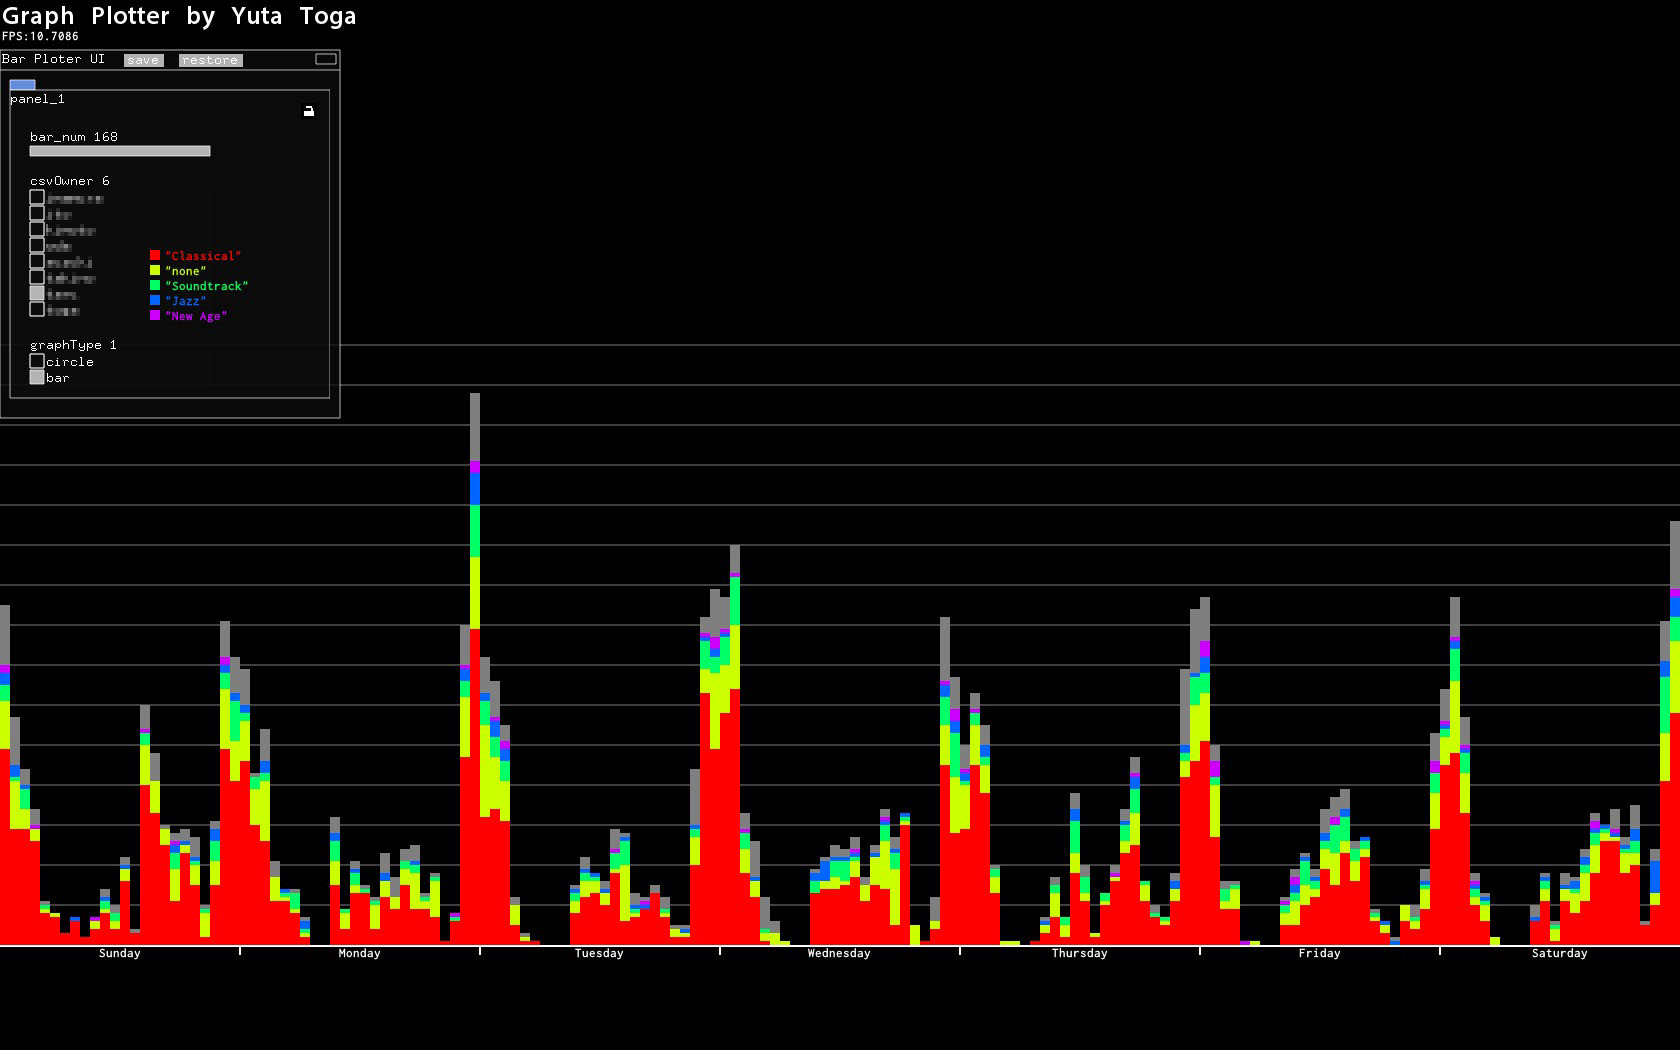
\includegraphics[width=14cm]{sample_regular.jpg}
\caption{規則的な人の例}
\label{sample_regular}
\end{center}
\end{figure}


\subsection{不規則な人}
不規則な人は、図\ref{sample_irregular}のグラフに示すように時間によって音楽の試聴のリズムは見られない。
曜日によって、ばらばらになっている。

\begin{figure}[h]
\begin{center}
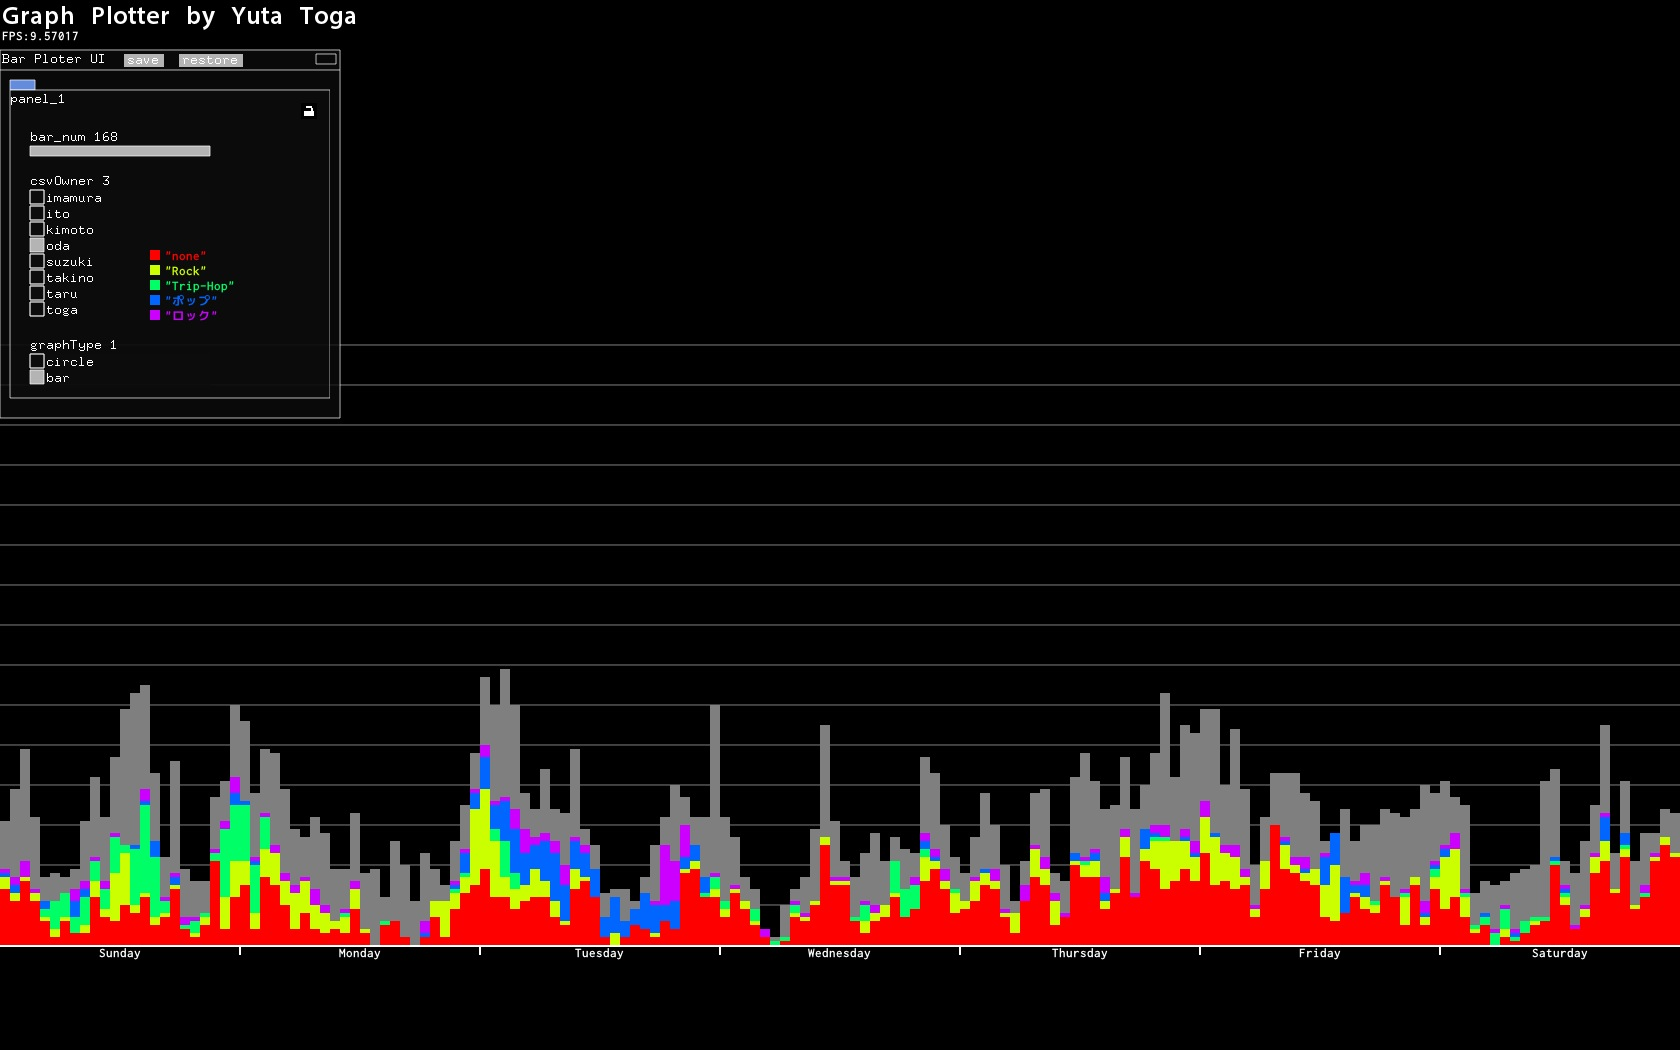
\includegraphics[width=14cm]{sample_irregular.jpg}
\caption{不規則な人の例}
\label{sample_irregular}
\end{center}
\end{figure}

\subsection{音楽ジャンルの分布が一定な人}
図\ref{genreMap_regular}のグラフに示すように、高さを見なかった場合、一定なパターンもある。それは、この場合、シャッフルプレイをしているために、iTunesに入っている音楽ライブラリのジャンル構成がそのまま音楽の再生の分布になっていると考えられる。

\begin{figure}[h]
\begin{center}
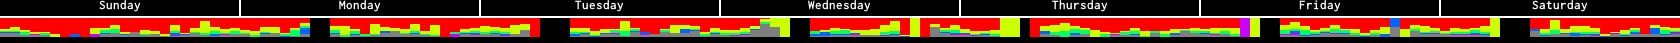
\includegraphics[width=14cm]{genreMap_regular.jpg}
\caption{音楽ジャンルの分布が一定な人の例}
\label{genreMap_regular}
\end{center}
\end{figure}


\subsection{音楽ジャンルの分布むらがある人}
\begin{figure}[h]
\begin{center}
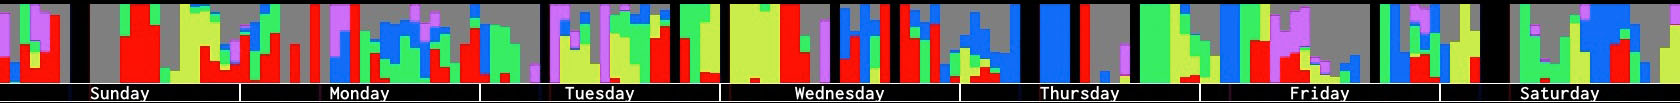
\includegraphics[width=14cm]{genreMap_irregular.jpg}
\caption{音楽ジャンルの分布にむらがある人の例}
\label{genreMap_irregular}
\end{center}
\end{figure}

\subsection{音楽をあまり聴かない人}
余り聞かない人は、曜日ごとのトップ5が占める比率も80%を超えることが多い。


\section{分析}
iTunesの仕様により、再生履歴は最後に聞いた時間の情報しか残っていない。すなわち、10回聞いたの楽曲がある場合も、いつ聞いたのかという情報は最後の10回目しか記録されておらず、1回目から9回目の情報は上書きによって失われている。そのため、今回の研究では、アンケートにおいて、シャッフルで再生しているかどうかを聞き出すことにした。
 もし、月曜日に特に音楽を聞いているという場合、なぜ月曜にそうなるのかという理由は聴いてみないとわからないため、アンケートで得られた、普段の生活を参照した。
また、この時間あなたは授業などで音楽を聴けない状況ではないですか?というようにインタビューによって利用者の音楽試聴状況を推測することができた。これは、今後、自動選曲システムにおいて、設定をすべてユーザーに任せるのではなく、もしかして、金曜の夜はあまりロックは聴かないですね?というような、質問形式で数問回答させることにより、ユーザーの音楽試聴状況に沿った選曲ができる(沿うことがよいリコメンドかどうかは別として)可能性を示唆する。
ランダムに再生している人と、時間と音楽再生に偏り(相関がある)人にどう分かれるのかを調べる。

\section{考察}
アンケートに書かれていることと、xmlファイルから得られた音楽再生の状況が異なる場合、一致する場合それぞれについて、なぜそうなるのかを考察する。
生活のコンテキスト、特に時間情報が音楽再生に影響力をもっているかどうかを考察し、音楽リコメンドサービスについての発展を考える。

寝ている間は聞いていない、授業に出ているときは聞いていないといった、特定の状況によって、音楽の再生が必ずされていない時間も存在することから、音楽の再生履歴だけで、そのひとの生活を推測することが出来る。また、音楽の聴き方は人によってばらつきがあり、特に、シャッフル機能を使っているかどうかによって、その差が大きく異なる。また、そもそもリコメンドサービスをするほどの情報を集められない人もおり、個人の情報による、個人のためのリコメンドサービスのためにはすくなくとも、いつでも音楽を多量に聴いている人という条件が必要である。そのため、音楽の余り聞かない人に音楽をリコメンドするためには、そのユーザーに音楽の好みを質問形式で聞いたり、音楽の聞く頻度や時間帯を質問するなどの問答を繰り返すことにより、リコメンドすべき時間やジャンルを推測する。その他の方法は、多くの人の音楽の聴き方を集めて、その人がどんな音楽再生のパターンをもっているのかを調べるのが良い。しかし、そのためには、その人が自分の音楽の聴き方を自分で把握している必要がある。今回の実験では、本人が自覚していないのにもかかわらず、定期的な音楽の聴き方をしている例も見られているため、自分で自分が聞きたいものを別の時間にすべて回答することは困難に思える。そのため、まずは従来の音楽の聴き方をして、その履歴から、次第にユーザーの好みを学習していくことが望ましい。本研究ではiTuensを使用したたが、第二章で述べたように履歴情報といっても欠落している情報が多く、ユーザーがスキップしたかどうかや、シャッフルプレイで再生したのかどうかや、ひとつの楽曲の履歴時間などを把握することができなかった。例えば、スキップしたとすると、ユーザーはその楽曲を積極的に聴きたくないという意志を表しているため、ユーザーの好みの学習には直接的に有効である。そのため、音楽再生プレイヤー自体がユーザーの好みを学習できるようにしておくべきである。そのためには、ユーザーが自分の操作を保存されること、第三者に自分の履歴情報を提供することなどプライバシーなどの問題もあるかもしれないが、煩雑な操作からの開放、聞きたかった音楽との出会いの推進のために進めていくことが望まれる。現在にいたっても単純なシャッフルプレイの人気を知ることになったが、リコメンドとはシャッフル以上のものであることが望まれるため、ユーザーの聞きたいものだけを推薦するだけでは単調になってしまうなどのことも考えられる。というのも、音楽の再生に偏りがあるひとも少なからず他の楽曲も聴いているからである、そのため、すべてをランダムにするわけでもないが、このみのジャンルを時間から推測し、ジャンルによって再生確立が動的に変化して、偏りのあるシャッフル再生にすることを提案したい。

\section{備考}
研究資料および、プログラムの一部は、(個人情報は含まない)
yutatoga.com/thesisからダウンロードできる。


\end{document}